\documentclass[conference]{IEEEtran}

\usepackage{amsmath,amssymb}
\usepackage{newtxtext,newtxmath}
\usepackage{booktabs}
\usepackage{graphicx}
\usepackage{microtype}
\usepackage{url}
\usepackage{xcolor}
\usepackage{balance}

% Permit two wide result floats to share a page before the discussion.  The
% defaults otherwise defer the biological diagnostic until after Conclusion.
\renewcommand{\dbltopfraction}{0.95}
\renewcommand{\dblfloatpagefraction}{0.85}
\setcounter{dbltopnumber}{2}

\graphicspath{{final_figures/}{figures/}}
\newcommand{\method}{StrataSCAN}
\newcommand{\R}{\mathbb{R}}
\newcommand{\ind}{\mathbb{I}}
\newcommand{\given}{\,\middle|\,}

\title{Description-Length Optimization of Density Strata on Sparse $k$-Nearest-Neighbor Graphs}

\author{\IEEEauthorblockN{Anonymous Author(s)}
\IEEEauthorblockA{Anonymous submission for triple-blind review}}

\begin{document}
\maketitle

\begin{abstract}
Clustering with several density levels and a dominant background is difficult because one radius may erase sparse clusters or connect dense clusters through background bridges. We present \method{} 0.2.4, a label-free sparse-graph method combining a multiscale Gamma mixture, exact within-stratum core-distance event sweeps, a coded background scan, and density-ordered non-merging growth. Evaluation uses Hungarian one-to-one target matching and retains failed-execution denominators. On 21 fresh synthetic cells, StrataSCAN completed every cell and achieved the highest mean target F1 (0.828) and discovery rate (0.827) among full-matrix completers. It discovered every target across 16--256-fold density contrasts and through 99\% low-density background, where target F1 was 0.979 and background F1 was 0.9996. StrataSCAN completed all seven families at one and two million observations and five at five million, and on 13 cytometry datasets it had the highest median target F1 among methods completing the full panel.
% FINAL-STATS: abstract
% After evidence freeze, add at most one synthetic effect sentence and one
% execution-envelope sentence from tables/final_statistical_summary.json; retain denominators.
% FINAL-STATS-BEGIN: abstract
On the fresh-seed block, joint-success StrataSCAN-minus-baseline mean one-to-one target-F1 effects ranged from +0.052 (HDBSCAN) to +0.741 (SNN-DBSCAN). The separate StrataSCAN-only execution envelope completed 26/28 prespecified cells.
% FINAL-STATS-END: abstract
\end{abstract}

\begin{IEEEkeywords}
variable-density clustering, minimum description length, $k$-nearest-neighbor graph, background rejection, graph optimization
\end{IEEEkeywords}

\section{Introduction}
Modern scientific datasets routinely contain millions of observations, clusters at different density levels, rare populations, and a dominant background. We seek a flat clustering with unknown cluster count that preserves locally supported populations, leaves unsupported observations unassigned, and remains practical at this scale.

The central difficulty is scale selection. DBSCAN uses one neighborhood radius~\cite{ester1996dbscan}, so a value suitable for a compact cluster can erase a diffuse one, while a larger value can create background bridges. Hierarchical and multi-density methods relax the single-radius assumption~\cite{ankerst1999optics,campello2013hdbscan,liu2007vdbscan,wang2022amd}, but a flat result still requires selecting an extraction level or searching over candidate parameter sets. On million-point data, repeated full-data searches are expensive and are often restricted to coarse grids or subsamples; either restriction can alter neighborhoods, rare populations, and the final partition. Graph community methods scale more naturally but usually assign every observation, whereas an explicit background/noise outcome is essential in our setting.

We develop \method, a label-free algorithm on a bounded-degree $k$NN graph. A multiscale Gamma model converts neighbor-shell volumes into ordered density strata and separates a model-derived background group. Within each supported stratum, candidate core structures are compared on a common description-length scale rather than selected by an externally tuned global radius. A separate scan can recover supported components from the background group, while density-ordered growth allows lower-density clusters to expand without merging identities already established at higher density. The construction is blockwise rather than a globally optimal joint program, and the all-background solution remains feasible.

This paper makes three contributions:
\begin{itemize}
  \item a multiscale Gamma/ICL model that maps $k$NN geometry to ordered density strata and an explicit model-derived background class;
  \item a sparse, label-free extraction algorithm that selects supported cluster structure, can abstain, and preserves established identities across density levels; and
  \item evidence that \method{} recovers clusters across 16--256-fold density contrasts, preserves rare dense targets through 99\% background, and executes on datasets containing up to five million observations.
\end{itemize}

The comparison panel follows the same task definition: it covers fixed-scale, hierarchical, shared-neighbor, multi-density, sparse-$k$NN, and graph-community families, but includes only configurations that can be run non-interactively under one frozen, label-free protocol. The implementation-level inclusion and exclusion criteria are stated in the experimental design.

Fig.~\ref{fig:pipeline} summarizes the computational path. Every production object is an array or bounded-degree sparse graph; dense pairwise distances are never materialized.

\begin{figure*}[t]
  \centering
  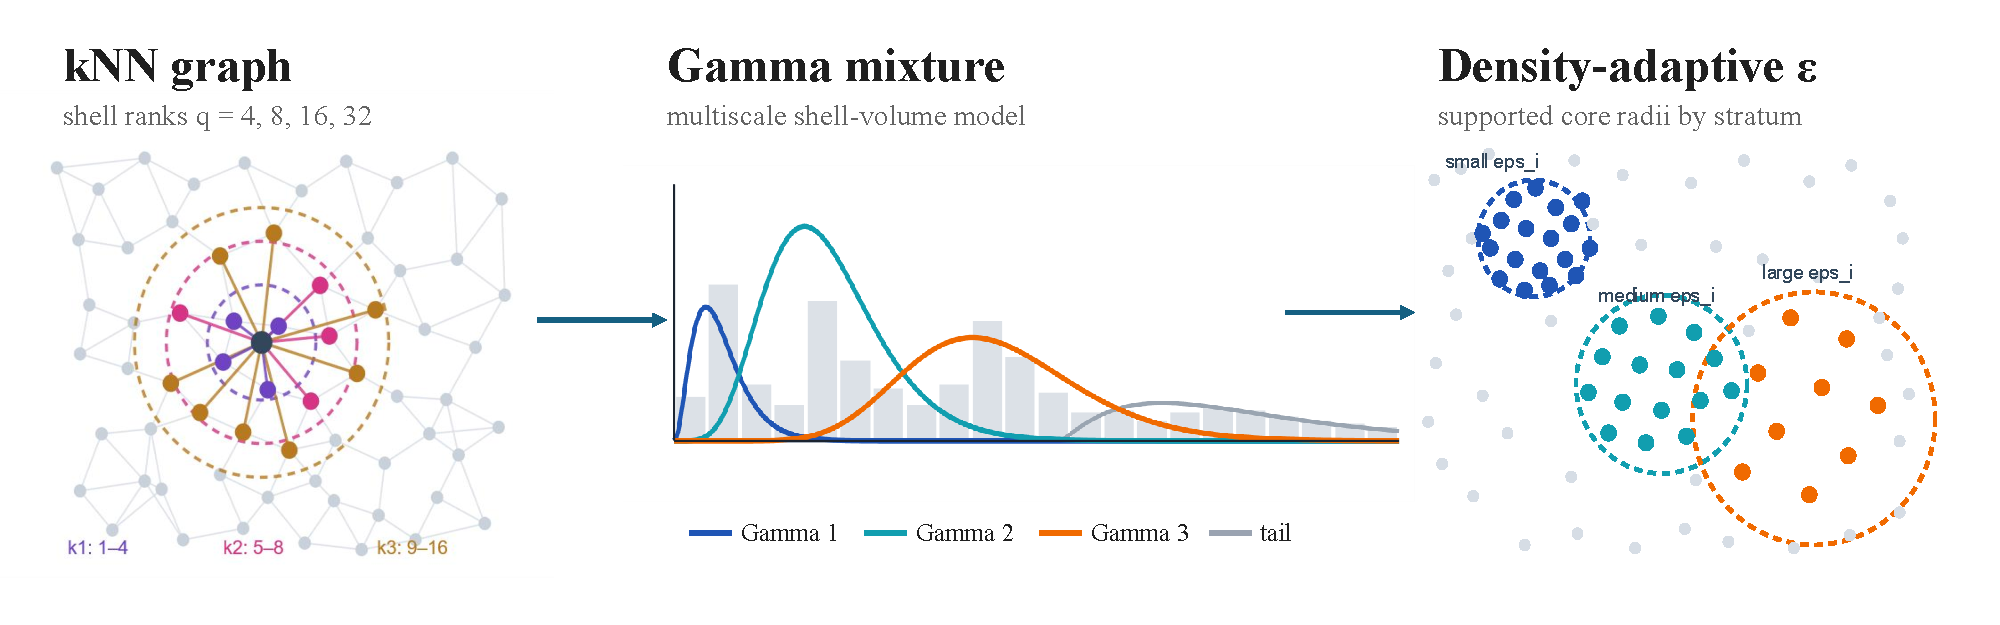
\includegraphics[width=\textwidth]{fig1_method_pipeline.pdf}
  \caption{\method{} pipeline and claim boundaries. The stages distinguish sparse geometry, adaptive density modeling, the exact within-stratum event sweep, the coded background search, and non-merging extraction. Annotations are used only during evaluation. The diagram states design properties and makes no empirical speed or accuracy claim.}
  \label{fig:pipeline}
\end{figure*}

\section{Related Work}
\textbf{Fixed-scale and multi-density clustering.}
DBSCAN provides arbitrary-shape clusters and an explicit noise label, but one $(\varepsilon,\mathrm{MinPts})$ pair defines a global density scale~\cite{ester1996dbscan}. Shared-nearest-neighbor variants replace metric distance by neighborhood overlap but still require a similarity scale~\cite{ertoz2003snn}. OPTICS and HDBSCAN construct density hierarchies~\cite{ankerst1999optics,campello2013hdbscan}; selecting a flat partition then requires a cut or stability rule. VDBSCAN and AMD-DBSCAN estimate multiple density-specific parameter sets~\cite{liu2007vdbscan,wang2022amd}. These approaches broaden the range of recoverable densities, but candidate enumeration or hierarchy extraction remains part of model selection and can be sensitive to the searched scales.

\textbf{Density peaks and graph partitions.}
Density Peaks and X-shift replace a global radius by assigning observations toward local density maxima~\cite{rodriguez2014dpc,samusik2016phenotype}. PhenoGraph constructs a shared-neighbor graph and applies community detection, while Leiden improves the connectivity of graph communities~\cite{levine2015aml,traag2019leiden}. FlowSOM uses a self-organizing map and metaclustering for fast cytometry analysis~\cite{vangassen2015flowsom}. These methods are important alternatives for heterogeneous data, but they still require choices such as a density estimator, peak or merge rule, graph resolution, or output cluster count. Graph and cytometry methods also commonly return a complete partition rather than an explicit model-derived background class. We therefore distinguish conceptual relevance from benchmark eligibility: a method can belong in this review yet remain outside the quantitative panel when no non-interactive cross-suite profile or validated implementation was frozen.

\textbf{Selection and scale.}
Nearest-neighbor radii are classical density statistics~\cite{loftsgaarden1965knn}, and HNSW/FAISS-style search makes bounded-degree $k$NN graphs practical in high dimensions~\cite{malkov2020hnsw,johnson2019faiss}. The graph alone, however, does not select density levels, extraction thresholds, or background semantics. Repeating clustering across many scales is costly on millions of observations, while subsampling can remove rare populations or change local connectivity. \method{} therefore constructs one sparse graph, aggregates disjoint neighbor-shell volumes with a Gamma/ICL model~\cite{biernacki2000icl}, and uses conditional description gain~\cite{rissanen1978mdl} to select supported structures. The density model and graph extraction remain separate: explaining density variation does not force every mixture component to become a cluster.

\section{Problem Statement}
Let $X=\{x_i\}_{i=1}^n\subset\R^d$. The desired output is $z_i\in\{-1,0,\ldots,K-1\}$, where $-1$ denotes background/noise and $K$ is unknown. Let $G_k=(V,E_k)$ be the directed $k$NN graph with neighbor distance $d_{i,q}$ at rank $q$. We require:
\begin{enumerate}
  \item all geometric decisions use edges already present in $G_k$;
  \item the all-background assignment is feasible;
  \item density levels may differ across output clusters;
  \item lower-density evidence cannot merge clusters already separated at higher density; and
  \item evaluation labels are unavailable to model and threshold selection.
\end{enumerate}

The present solver is a blockwise optimization. First it chooses a Gamma density model $M$. Given $M$, it chooses supported density strata and core thresholds. Given the core set, it constructs identities and border/noise assignments. Each accepted core structure has positive description gain, but the complete pipeline is not claimed to solve a single joint nonconvex program to global optimality.

\section{Method}
\subsection{Multiscale Shell-Volume Mixture}
For ranks $0=q_0<q_1<\cdots<q_J=k$, define the shell-volume observation
\begin{equation}
 y_{ij}=c_d\left(d_{i,q_j}^{d}-d_{i,q_{j-1}}^{d}\right),
 \qquad a_j=q_j-q_{j-1},
 \label{eq:shell}
\end{equation}
where $c_d$ is the unit-ball volume. Conditional on density component $s$, the locally Poisson approximation gives
\begin{equation}
 p(y_{ij}\mid s)=\operatorname{Gamma}(y_{ij};a_j,\lambda_{sj}),
 \quad \log\lambda_{sj}=\mu_s+\beta_s\log q_j.
 \label{eq:gamma}
\end{equation}
The log-linear rate constraint couples scales and uses two continuous parameters per component instead of one unrelated rate per shell. With mixture weights $\pi_s$, EM estimates $\Theta_m=\{\pi_s,\mu_s,\beta_s\}_{s=1}^{m}$ on all observations. StrataSCAN 0.2.4 searches from $m=1$ through an initial bound of 8 and may expand in steps of four to a hard bound of 24. The ordinary search uses a deterministic cold start at $m=1$ and split-warm continuation between adjacent orders at relative tolerance $10^{-4}$. Specified high-order ambiguity patterns trigger a tighter guarded search: duplicate profiles restrict it to the selected order and its immediate neighbors, while other cases repeat the full candidate range. Split-warm continuation is disabled during confirmation, so every confirmed order uses independent cold initialization; the single-signal case uses two starts. Guarded confirmation changes neither the core objective nor the subsequent exact event sweep.

Let $r_{is}=p(s\mid y_i,\Theta_m)$. We choose
\begin{equation}
 m^*=\arg\min_m\left[-2\ell(\Theta_m)+p_m\log n+2H(R_m)\right],
 \label{eq:icl}
\end{equation}
where $p_m=(m-1)+2m$ and $H(R_m)=-\sum_{i,s}r_{is}\log r_{is}$. Equation~\eqref{eq:icl} is ICL in minimization form. Components are ordered by first-shell rate. In the evaluated version, the largest adjacent log-rate gap separates supported density strata from an explicit background group. A vertex receives its maximum-posterior component; its background posterior $b_i$ is the summed responsibility of background components. Thus the pointwise description gain of signal over background is
\begin{equation}
 u_i=\log\frac{1-b_i}{b_i}.
 \label{eq:unary}
\end{equation}

This semantic split is a limitation: the largest rate gap can underselect signal when true cluster and field densities overlap. We retain it in the locked method because replacing it after inspecting the final labels would invalidate the evaluation.

\subsection{Topology Code and Exact Core-Threshold Sweep}
For each non-background stratum $s$, sort its vertices by $\delta_i=d_{i,4}$. Every prefix $P_s(t)$ is a candidate strict core, so the threshold is always an observed distance. The first four neighbor slots construct connectivity; slots five through eight provide disjoint topology evidence, avoiding the tautology of scoring a component using the same edges that created it.

For a candidate set $C$ of size $a$, let $e_C$ be the number of held-out directed edges whose endpoint remains in $C$, and $T=4a$. Under a uniformly mixed reference, $p_0=(a-1)/(n-1)$. We integrate the alternative edge probability with a Jeffreys $\operatorname{Beta}(1/2,1/2)$ prior:
\begin{align}
 \log \mathrm{BF}(C)={}&\log\frac{B(e_C+\tfrac12,T-e_C+\tfrac12)}{B(\tfrac12,\tfrac12)} \nonumber\\
 &-e_C\log p_0-(T-e_C)\log(1-p_0).
 \label{eq:bf}
\end{align}
Candidates no denser than the null receive gain $-\infty$. The stratum-prefix gain is
\begin{equation}
 G_s(t)=\sum_{i\in P_s(t)}u_i+\log\mathrm{BF}(P_s(t))-\log |V_s|.
 \label{eq:prefix}
\end{equation}
The final term is the implementation's uniform code over the $|V_s|$ candidate activation events within the current stratum; it is not a global $\log n$ threshold code. As vertices activate in sorted order, cumulative unary gain and held-out edge count update incrementally. We evaluate every event and take $t_s^*=\arg\max_t\max(0,G_s(t))$ exactly. Because $k$NN edges are dependent, $\log\mathrm{BF}$ is an integrated edge-surprisal score, not a calibrated Bayes factor for the complete clustering; the summed objective is MDL-inspired rather than a proof of a joint universal code.

The selected prefix can contain several connected components. For component $C$, we recompute held-out topology evidence and retain it only if
\begin{equation}
 G(C)=\sum_{i\in C}u_i+\log\mathrm{BF}(C)-\log n>0,
 \label{eq:component}
\end{equation}
where $\log n$ is a uniform code for one representative root. This removes the need for a fixed minimum cluster size: a small component is permitted if its density and topology repay its identity.

\subsection{Coded Search Inside the Background}
A sparse cluster may lie inside the Gamma background group. We therefore apply the same core concept through an adaptive scan rather than a fixed ``tail'' fraction. Background vertices are ordered by $d_{i,4}$. Candidate prefix widths are dyadic, $w\in\{4,8,16,\ldots\}$, up to half of the active background. For each $w$, the largest connected component in the first rank window is compared with equally sized later windows. Its smoothed empirical tail probability is
\begin{equation}
 \hat p_w=\frac{1+\#\{j>1:A_j\ge A_1\}}{J_w}.
\end{equation}
The activation gain $-\log\hat p_w-\log|\mathcal W|-\log 2$ pays for the width search and activate/skip decision. A candidate must additionally repay a Poisson/Beta boundary code and the graph code
\begin{equation}
 L_{\mathrm{graph}}=\log |B|+(|C|-1)\log 4+\log|\mathcal W|.
\end{equation}
Only positive net-gain components are removed from the active background and the process repeats. There is no fixed tail mass, quantile, or $p$-value cutoff; however, repeated adaptive scans do not provide a formal family-wise error guarantee and remain a future sensitivity target.

\subsection{Density-Ordered Extraction and Border Decisions}
Core strata are processed from high to low Gamma rate. Within one stratum, directed graph edges are admitted only when their metric length does not exceed the source core radius $\varepsilon_s=d_{(t_s^*),4}$. A core component without contact to an earlier stratum creates a new cluster. If it contacts existing denser clusters, multi-source shortest-path growth assigns its vertices to those seeds; it may extend, but never merge, the existing identities. This is a density-ordered, non-merging graph watershed.

For a non-core vertex $i$, consider its first four graph neighbors that already have cluster labels. It attaches through the neighbor minimizing $d_{ij}/\varepsilon_{s(j)}$ only if that ratio is at most one. Otherwise $z_i=-1$. The rule is deliberately conservative: no global border multiplier and no post-hoc forced assignment are used.

\subsection{Conditional Guarantees}
The blockwise construction does not imply global optimality, but two useful guarantees hold inside its declared search space.

\textbf{Proposition 1 (event-sweep optimality).} Fix a fitted mixture, one stratum $V_s$, its unary gains, the graph slots assigned to topology scoring, and a deterministic ordering of equal distances. The threshold $t_s^*$ maximizes~\eqref{eq:prefix} over every core set induced by an observed fourth-neighbor-distance event, including the empty core.

\emph{Proof sketch.} Between consecutive observed distances, the strict core set is unchanged. Activating vertices in sorted order therefore enumerates every distinct candidate in this conditional family. The unary sum and held-out edge count are sufficient statistics for~\eqref{eq:prefix}; updating both at each event and retaining the largest nonnegative value returns its maximum. The outer maximum with zero explicitly represents the empty core. $\square$

\textbf{Proposition 2 (non-merging invariant).} After a denser stratum has created cluster identities, processing any lower-density stratum cannot merge two of those identities.

\emph{Proof sketch.} A lower-density component with no earlier contact receives a new identity. With one or more earlier contacts, multi-source growth assigns each new vertex to exactly one existing seed under deterministic distance and identifier tie-breaking. The update adds vertices to seed labels but never rewrites an earlier labeled vertex or unions seed identifiers. Strict-radius border assignment has the same one-label update. Induction over strata and border vertices proves the claim. $\square$

These guarantees isolate what is exact and stable from what remains model-dependent: mixture selection, the largest-rate-gap semantic split, and the background scan are conditional modeling blocks rather than parts of a joint optimum.

\subsection{Complexity}
With fixed $k$, $J$, and candidate component cap $m_{\max}$, shell construction and EM storage are $O(nk+nm_{\max})$. Mixture fitting is $O(InJm_{\max})$ for $I$ EM iterations across candidates. Sorting core events costs $O(n\log n)$ in aggregate; edge scans, connected components, watershed growth, and border decisions use $O(nk)$ sparse state. Approximate neighbor construction dominates geometry at high dimension. The method therefore avoids $O(n^2)$ storage, although fitting every row for every ICL candidate is a significant runtime cost.

\section{Experimental Design}
\subsection{Datasets and Preprocessing}
\textbf{Synthetic data.} Seven generators cover multi-density blobs, 95\% noise in 16 dimensions, overlapping density, moons, rings, Gaussian overlap, and severe imbalance. The canonical all-method release block contains 504 native 0.2.4 cells at $n=20{,}000$: five development seeds and three fresh seeds, analyzed separately. A 27-cell StrataSCAN campaign varies determinant-defined target-density contrast from 16 to 256, and a separate 270-cell all-method campaign holds three dense 100-point targets fixed while low-density background rises from 25\% to 99\%. Large-$n$ evidence contains seven families at 0.5, one, two, and five million observations.

\textbf{Biological data.} We evaluate Levine, Mosmann, and Nilsson benchmark cytometry data and ten independently processed Samusik mouse samples~\cite{levine2015aml,samusik2016phenotype,weber2016cytometry}. Together they contain 1,547,871 cells, 7--39 type markers per dataset, and expert population annotations plus an unassigned/background class. Type-marker intensities receive the predeclared arcsinh transform (cofactor 5 for Levine and Samusik; 150 for Mosmann and Nilsson) followed by robust median/MAD scaling.


\subsection{Baselines and Protocol}
The panel was selected by algorithmic role rather than as an exhaustive list of published software. Eligibility required a method to fit without reference labels, return a flat point partition accepted by the shared evaluator, run non-interactively under the same resource monitor, and use an inspectable implementation and parameter profile frozen before evaluation. DBSCAN is the fixed-scale density control; OPTICS and HDBSCAN represent hierarchical density adaptation; SNN-DBSCAN tests shared-neighbor similarity; VDBSCAN-2007 represents explicit multi-density parameterization; $k$NN-DBSCAN is a $k$NN-informed scale control; and $k$NN+Leiden is an all-assigned graph-community control. This provides coverage of the relevant failure modes---global scale, hierarchy extraction, multiple-density search, graph partitioning, and lack of abstention---without claiming that the selected implementation is universally strongest within each family.

The reported panel is therefore DBSCAN, HDBSCAN, OPTICS, SNN-DBSCAN, VDBSCAN-2007, $k$NN-DBSCAN, $k$NN+Leiden, and StrataSCAN 0.2.4. DBSCAN/HDBSCAN/OPTICS use scikit-learn~\cite{pedregosa2011sklearn}; the remaining baselines are controlled implementations, so their names identify declared algorithmic profiles rather than official author software. Methods requiring an analyst-selected cut, center set, or output cluster count were not admitted unless an automatic rule had been fixed in advance. Consequently, original Density Peaks was not benchmarked because its decision graph introduces a center-selection step~\cite{rodriguez2014dpc}; X-shift is confined to a focused Nilsson sensitivity because our available controlled port and its automatic $K$ rule were not validated as a cross-suite profile~\cite{samusik2016phenotype}; and FlowSOM was not added because no cross-suite output-cluster-count rule had been frozen before evaluation~\cite{vangassen2015flowsom}. The $k$NN+Leiden control covers the graph-community mechanism but is not presented as a reproduction of PhenoGraph~\cite{levine2015aml}. These are automation, scope, and provenance exclusions, not evidence that the omitted methods are intrinsically inferior.

A preliminary artifact labeled \texttt{AMD-DBSCAN} was an AMD-inspired surrogate rather than an official-compatible port~\cite{wang2022amd}; it also retained a dense pairwise-distance stage that exceeded the 8-GiB limit on the cytometry inputs. It is documented for provenance but excluded from all comparative Results. Synthetic release, rare-dense, and cytometry predictions are native executions under frozen method profiles. StrataSCAN 0.2.4 uses the adaptive 8--24 component search and guarded confirmation described above. Historical predecessor and model-perturbation results are excluded from submission claims.

The same eight reported methods are evaluated on synthetic and cytometry blocks under the frozen \texttt{target-discovery-v1} contract. Every successful row records Hungarian maximum-F1 matching, equal-target aggregation, purity threshold 0.90, coverage threshold 0.10, suite-specific background semantics, and its evaluation generation. Failed executions retain missing quality and remain in completion denominators; runtime and process peak RSS use successful executions only. Inputs with absent or mismatched evaluator metadata are rejected rather than combined. Stochastic biological repetitions are collapsed within dataset and method before cross-dataset summaries.

\subsection{Metrics and Statistics}
Let $T_1,\ldots,T_R$ be reference targets and $C_1,\ldots,C_K$ predicted non-background clusters. For every pair, purity is $P_{rk}=|T_r\cap C_k|/|C_k|$, coverage is $Q_{rk}=|T_r\cap C_k|/|T_r|$, and $F_{rk}=2P_{rk}Q_{rk}/(P_{rk}+Q_{rk})$. Hungarian assignment maximizes $\sum_r F_{r,\pi(r)}$ subject to one-to-one target--cluster matching; unmatched targets receive zero. The primary target score is the equal-target mean $F_T=R^{-1}\sum_r F_{r,\pi(r)}$. We also report macro purity and coverage, and call a target discovered only when its assigned cluster has purity $\geq0.90$ and coverage $\geq0.10$. The thresholds were locked for this revision before the canonical rescore and are not optimized per dataset.

Candidate burden reports predicted, matched, unmatched, background-only, and background-majority cluster counts. Synthetic data additionally provide true-noise F1 and full-partition pairwise F1. For cytometry, binary agreement between reference negatives and predicted abstention is labeled a \emph{background-abstention diagnostic}; reference negatives are not asserted to be physical noise, and no harmonic composite is used for ranking.

Dataset-level summaries retain all 13 biological datasets and every named comparator. Because ten Samusik samples come from one benchmark study, we show both an equal-dataset summary and a dependence-aware sensitivity that first averages Samusik 01--10 and then weights Samusik, Levine, Mosmann, and Nilsson equally. The weighting scheme was not predeclared, so neither aggregation is treated as confirmatory and their ranking difference remains visible. Synthetic bootstrap intervals summarize paired mean effects descriptively; no multiplicity-controlled hypothesis test or population-level confidence interpretation is claimed. No diagnostic changes the recorded predictions.

\section{Results}
We organize the evidence around four research questions. All quality values use one-to-one target matching; failures remain in completion denominators and never receive fabricated zero scores.

\subsection{RQ1: Recovery Across Synthetic Structures}
\textbf{Does StrataSCAN provide competitive target recovery across heterogeneous synthetic datasets?}
The fresh panel contains three prespecified seeds for each of seven families (21 cells per method); the five development seeds remain separate. StrataSCAN completed all 21 fresh cells with mean target F1 $0.828\pm0.263$ and mean discovery rate 0.827 (Table~\ref{tab:synthetic-fresh}). Among the reported methods, these were the highest mean F1 and discovery rate. Cell-wise paired median F1 differences favored StrataSCAN against six of seven baselines, ranging from +0.065 against VDBSCAN-2007 to +0.870 against SNN-DBSCAN. HDBSCAN retained a small paired median advantage of 0.007, so the result supports broad competitive recovery rather than dominance on every family.

\begin{table}[t]
\centering
\caption{Synthetic target recovery on three fresh seeds across seven families.}
\label{tab:synthetic-fresh}
\setlength{\tabcolsep}{4.2pt}
\begin{tabular}{lcc}
\toprule
Method & Target F1 & Discovery \\
\midrule
\textbf{StrataSCAN} & \textbf{$0.828\pm0.263$} & \textbf{0.827} \\
HDBSCAN & $0.776\pm0.330$ & 0.603 \\
VDBSCAN-2007 & $0.671\pm0.328$ & 0.579 \\
$k$NN+Leiden & $0.619\pm0.267$ & 0.357 \\
DBSCAN & $0.551\pm0.323$ & 0.563 \\
$k$NN-DBSCAN & $0.539\pm0.369$ & 0.540 \\
OPTICS & $0.374\pm0.354$ & 0.347 \\
SNN-DBSCAN & $0.087\pm0.104$ & 0.159 \\
\bottomrule
\end{tabular}
\begin{minipage}{0.98\columnwidth}\footnotesize Target F1 is the mean $\pm$ sample SD across 21 fresh cells. Discovery is the mean fraction of reference targets matched at purity $\geq0.90$ and coverage $\geq0.10$.\end{minipage}
\end{table}


% FINAL-STATS: synthetic-contrasts
% FINAL-STATS-BEGIN: synthetic-contrasts
Under Hungarian one-to-one matching, Development effects ranged from +0.051 (HDBSCAN) to +0.734 (SNN-DBSCAN). Joint-success coverage was 35/35 for DBSCAN, HDBSCAN, OPTICS, SNN-DBSCAN, VDBSCAN-2007, kNN+Leiden, kNN-DBSCAN. Fresh-seed effects ranged from +0.052 (HDBSCAN) to +0.741 (SNN-DBSCAN). Joint-success coverage was 21/21 for DBSCAN, HDBSCAN, OPTICS, SNN-DBSCAN, VDBSCAN-2007, kNN+Leiden, kNN-DBSCAN. Failed pairs remain in completion counts but do not receive fabricated quality scores.
% FINAL-STATS-END: synthetic-contrasts

\subsection{RQ2: Density Contrast and Dominant Background}
\textbf{Can StrataSCAN recover clusters with strongly varying densities and preserve rare dense targets under extreme background contamination?}
We first varied the peak density among six equal-mass Gaussian targets while holding target count, separation, and 25\% background fixed. The 27-cell StrataSCAN campaign covered density ratios 16, 64, and 256 in 2D and 8D with isotropic and rotated anisotropic targets. All cells completed, every target met the 0.90-purity/0.10-coverage discovery rule, and the nine case medians ranged from 0.829 to 0.929 target F1 [Fig.~\ref{fig:density-noise}(a)]. Because the 243-cell baseline density matrix was not executed, this panel establishes capability rather than comparative superiority.

We then fixed three dense 100-point targets and increased low-density background from 25\% to 99\%, preserving an empirical 16-neighbor signal/background density ratio of approximately 8.4--17.2. The all-method design retained 270 attempted cells; 268 completed. StrataSCAN completed 30/30 cells, discovered every target at every level, and maintained level-wise median target F1 between 0.852 and 0.981 [Fig.~\ref{fig:density-noise}(b)]. At 99\% background it obtained target F1 0.979 and background F1 0.9996, the best background rejection in the panel; no comparator exceeded it on both endpoints (Table~\ref{tab:rare-dense-99}).

\begin{figure*}[t]
  \centering
  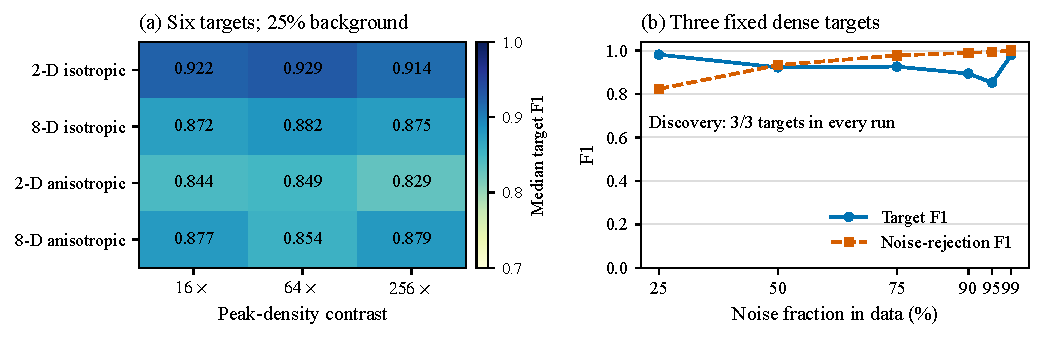
\includegraphics[width=0.985\textwidth]{fig2_density_noise.pdf}
  \caption{Density adaptation and rare-target recovery. (a) Each tested cell gives StrataSCAN's three-seed median target F1 for the stated dimensionality, geometry, and determinant-defined peak-density ratio; blank cells were not tested. This density matrix is StrataSCAN-only. (b) Median target and known-background F1 as low-density background rises around three fixed dense targets; whiskers show the five-seed range. Every target satisfied the locked discovery rule in every run.}
  \label{fig:density-noise}
\end{figure*}

\begin{table}[t]
\centering
\caption{Recovery at 99\% low-density background. Medians over five paired seeds.}
\label{tab:rare-dense-99}
\setlength{\tabcolsep}{4.5pt}
\begin{tabular}{lcc}
\toprule
Method & Target F1 & Background F1 \\
\midrule
\textbf{StrataSCAN} & \textbf{0.979} & \textbf{1.000} \\
HDBSCAN & 1.000 & 0.000 \\
VDBSCAN-2007 & 1.000 & 0.029 \\
$k$NN+Leiden & 1.000 & 0.000 \\
DBSCAN & 0.995 & 0.487 \\
$k$NN-DBSCAN & 0.986 & 0.673 \\
OPTICS & 0.943 & 0.994 \\
SNN-DBSCAN & 0.992 & 0.115 \\
\bottomrule
\end{tabular}
\end{table}


\subsection{RQ3: Million-Scale Execution}
\textbf{Does StrataSCAN remain computationally practical on datasets containing millions of observations?}
Under one thread, a 3,600-s timeout, and an 8-GiB process limit, the complete 28-cell StrataSCAN campaign covered seven families at 0.5, one, two, and five million observations. StrataSCAN completed 7/7 families at one million, 7/7 at two million, and 5/7 at five million (Fig.~\ref{fig:million-scale}). Median successful-run runtime increased from 4.00 to 8.17 and 23.07 min; median five-million-point peak RSS was 6.29 GiB. Rings and 8-D Gaussian overlap reached the memory limit. At five million, imbalanced, ultrasparse, and moons retained target F1 0.949, 0.995, and 0.811 with discovery 1.0, whereas multidensity and overlapping-density remained weaker and are not used for a universal quality claim.

The baseline ladder is complete at the shared one- and two-million sizes but structurally incomplete at five million (177/224 expected records) and contains no scaling-quality fields. StrataSCAN and $k$NN-DBSCAN were the only methods completing all seven families at both one and two million (Table~\ref{tab:million-scale}). In the one directly matched five-million-point imbalanced case, StrataSCAN completed in 30.64 min, versus 34.39 min for $k$NN-DBSCAN and 36.20 min for SNN-DBSCAN; $k$NN+Leiden reached the memory limit. These results demonstrate a broad million-scale execution envelope, not universal raw-speed superiority.

\begin{figure}[t]
  \centering
  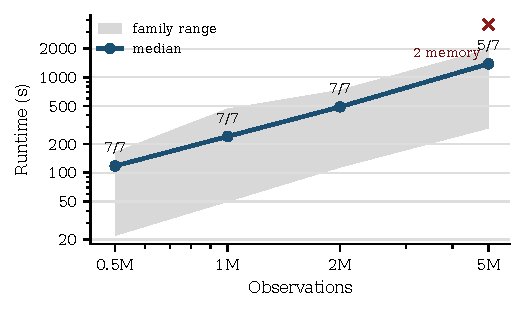
\includegraphics[width=\columnwidth]{fig3_million_scale.pdf}
  \caption{StrataSCAN runtime across seven synthetic families under one thread, a 3,600-s timeout, and an 8-GiB process limit. The line is the successful-run median, the band is the family range, and labels report completion. Failed jobs receive no artificial runtime.}
  \label{fig:million-scale}
\end{figure}

\begin{table}[t]
\caption{Million-scale completion and successful-run runtime.}
\label{tab:million-scale}
\centering
\footnotesize
\setlength{\tabcolsep}{2.7pt}
\begin{tabular}{@{}lrrrr@{}}
\toprule
Method & 1M & 2M & 5M & 2M time (s)\\
\midrule
\textbf{StrataSCAN} & \textbf{7/7} & \textbf{7/7} & \textbf{5/7} & 490\\
DBSCAN & 6/7 & 3/7 & P$^{*}$ & 58\\
HDBSCAN & 0/7 & 0/7 & P$^{*}$ & --\\
OPTICS & 0/7 & 0/7 & P$^{*}$ & --\\
SNN-DBSCAN & 7/7 & 6/7 & 1/1$^{*}$ & 355\\
VDBSCAN-2007 & 4/7 & 3/7 & P$^{*}$ & 75\\
$k$NN-DBSCAN & 7/7 & 7/7 & 1/1$^{*}$ & 331\\
$k$NN+Leiden & 5/7 & 1/7 & M$^{*}$ & 1042\\
\bottomrule
\multicolumn{5}{p{0.95\columnwidth}}{\scriptsize Done/recorded families. $^{*}$The baseline 5M ladder is incomplete; M is memory limit and P is a gated skip. Times are medians over successes.}
\end{tabular}
\end{table}


% FINAL-STATS: scaling-envelope
% FINAL-STATS-BEGIN: scaling-envelope
StrataSCAN completed 26/28 cells. At 5,000,000 observations, successful-family runtime ranged from 294 to 1961~s and per-process RSS from 5648 to 7848~MiB.
% FINAL-STATS-END: scaling-envelope

\subsection{RQ4: Transfer to Cytometry}
\textbf{Does StrataSCAN generalize from controlled synthetic datasets to real cytometry data?}
The reported native matrix contains 104 attempted cells across 13 datasets and eight methods; 99 completed. StrataSCAN completed 13/13 datasets and obtained median target F1 0.202 (IQR 0.008--0.244), the highest median among methods completing the full panel (Fig.~\ref{fig:cytometry}). It led Levine (0.190 versus 0.036 for the best successful baseline) and Nilsson (0.517 versus 0.133), with median purity 0.437 and coverage 0.244. $k$NN+Leiden had the higher successful-run median F1 (0.284) and led all ten Samusik samples, but timed out on Levine and Mosmann and completed 11/13; its median purity was 0.225. SNN-DBSCAN was strongest on Mosmann and had the largest mean discovery rate. Thus, StrataSCAN's transfer advantage is reliability- and purity-oriented rather than universal across biological datasets.

An exploratory oversegmentation-tolerant sensitivity assigned each predicted component to at most one target and then merged components per target. It increased StrataSCAN's median F1 only from 0.202 to 0.221, so it did not resolve the low absolute scores and was not substituted for the locked one-to-one endpoint.
Because the ten Samusik samples belong to one study, an equal-study sensitivity first averages them and then weights Samusik, Levine, Mosmann, and Nilsson equally. Under that aggregation StrataSCAN ranked first of eight by target F1; the equal-dataset view and its different ranking remain visible rather than being pooled.

\begin{figure*}[t]
  \centering
  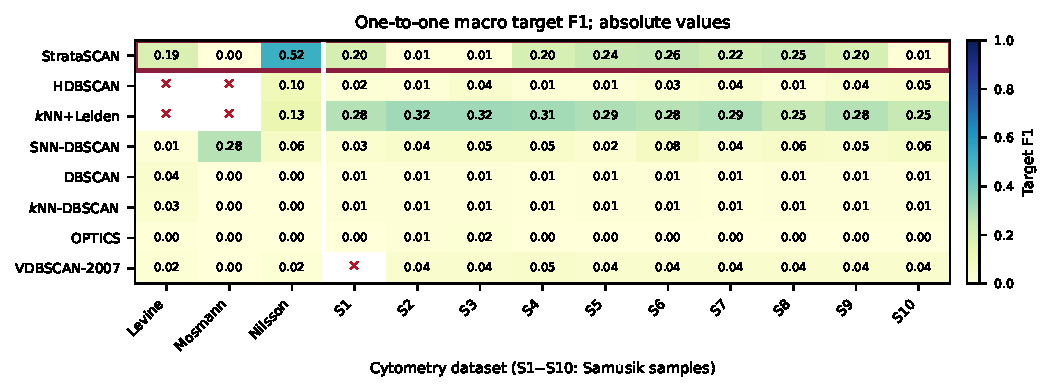
\includegraphics[width=0.985\textwidth]{fig4_cytometry.pdf}
  \caption{Dataset-resolved one-to-one macro target F1 across 13 cytometry datasets. Each cell reports the absolute score; crosses denote failed executions, which remain missing rather than becoming zero. The outlined row is StrataSCAN, and S1--S10 are the Samusik samples.}
  \label{fig:cytometry}
\end{figure*}

% FINAL-STATS: biological
% FINAL-STATS-BEGIN: biological
Under equal-study weighting, StrataSCAN ranked 1/9 by one-to-one target F1. Its target F1/purity/coverage/discovery rate was 0.217/0.288/0.472/0.011; background-abstention F1 was 0.336 (diagnostic). Successful-dataset coverage was 13/13.
% FINAL-STATS-END: biological

% Retain legacy synchronization anchors without exposing excluded result blocks.
\iffalse
% FINAL-STATS: noise-sensitivity
% FINAL-STATS-BEGIN: noise-sensitivity
The 270-cell controlled synthetic-noise factorial reports median one-to-one target F1/discovery rate/true-noise F1 for released StrataSCAN as 50\%: 0.970/1.000/0.969, 75\%: 0.926/0.000/0.974, 90\%: 0.822/0.000/0.978, 95\%: 0.708/0.000/0.979, 97.5\%: 0.338/0.000/0.979, 99\%: 0.005/0.000/0.031.
% FINAL-STATS-END: noise-sensitivity
% FINAL-STATS: gaia
% FINAL-STATS-BEGIN: gaia
Native 0.2.4 StrataSCAN completed 359/359 fields and discovered 330/359 fields at purity $\geq0.90$ and coverage $\geq0.10$. Successful-field median target F1/purity/coverage was 0.983/1.000/0.991; median unmatched candidate clusters was 7.0.
% FINAL-STATS-END: gaia
\fi
\section{Discussion and Limitations}
The four research questions expose complementary strengths rather than one aggregate rank. Fresh synthetic evidence establishes broad recovery; controlled density and background experiments isolate the method's intended regime; scaling measures the implementation at million-point sizes; and cytometry tests transfer without label-specific tuning. StrataSCAN led full-completion methods on fresh mean target F1 and discovery, rejected 99\% low-density background while preserving every rare target, completed every family at one and two million observations, and completed all 13 cytometry datasets.

One-to-one matching prevents two reference targets from receiving credit for the same predicted cluster, but no scalar certifies a complete partition. Purity, coverage, discovery, completion, and candidate burden therefore remain visible. Equal-dataset and equal-study cytometry summaries answer different questions: $k$NN+Leiden leads the Samusik-dominated equal-dataset view but misses two datasets, whereas StrataSCAN leads the dependence-aware equal-study F1 sensitivity and completes the full panel. Cytometry reference negatives can contain legitimate structure, so abstention agreement remains diagnostic rather than physical-noise accuracy.

There are six methodological limitations. First, the evaluated pipeline is blockwise rather than a globally optimized MDL program; its dependent-edge topology score is a composite codelength heuristic. Second, the largest Gamma rate gap can fail when signal density overlaps a background continuum. In the older local-overlap stress test, the 99\% endpoint simultaneously reduced each target to 100 observations and collapsed the local density ratio to about 1.18:1; StrataSCAN failed there, so the positive 99\% result is explicitly limited to rare targets that remain distinctly denser than their surroundings. Third, the Poisson shell model can be misspecified on lower-dimensional manifolds. Fourth, the density-contrast campaign is StrataSCAN-only and leaves residual fragmentation, so it demonstrates capability rather than baseline superiority. Fifth, the five-million baseline ladder is incomplete, two StrataSCAN families reached the 8-GiB limit, and completed-family quality varied. Sixth, the large-scale envelope uses one seed per family and characterizes measured execution rather than hardware-independent asymptotics.

Synthetic release, rare-dense, and cytometry comparisons use native 0.2.4 predictions for all eight reported methods. The artifact records protocol and result hashes, software environments, completion denominators, and scripts that reproduce the source tables. Missing measurements remain distinct from protocol-defined failures. Density contrast and scaling retain their narrower, explicitly stated evidence boundaries rather than being pooled with the all-method panels.

% FINAL-STATS: discussion
% After evidence freeze, add a short synthesis of the strongest
% supported positive and negative findings. Every value must come from
% tables/final_statistical_summary.json and preserve its analysis boundary.
% FINAL-STATS-BEGIN: discussion
Fresh-seed one-to-one target-F1 effects ranged from +0.052 to +0.741 across named baselines. Target recovery, discovery, candidate burden, and abstention diagnostics expose distinct trade-offs and do not support a universal ranking.
% FINAL-STATS-END: discussion

\section{Conclusion}
\method{} 0.2.4 replaces several quality-critical density thresholds with label-free conditional codelength decisions on a sparse $k$NN graph. Across four research questions, it combines strong full-matrix synthetic recovery, adaptation over 16--256-fold density contrast, rare-target recovery through 99\% low-density background, execution through five million observations, and complete cytometry coverage. The evidence does not imply universal dominance: HDBSCAN retains a small fresh-seed median advantage, the baseline five-million ladder is incomplete, and biological leadership depends on dataset aggregation. The supported conclusion is nevertheless positive and specific: StrataSCAN is a practical density-adaptive option when heterogeneous densities, explicit background rejection, and million-scale execution must be addressed together.

% FINAL-STATS: conclusion
% Optionally add one final evidence sentence after the freeze; do
% not turn it into a universal synthetic, biological, Gaia, or scaling claim.
% FINAL-STATS-BEGIN: conclusion
The target-discovery-v1 evaluation uses one-to-one matching and retains failed executions without fabricated quality; the separate execution envelope completed 26/28 cells.
% FINAL-STATS-END: conclusion

\balance
\bibliographystyle{IEEEtran}
\bibliography{references}

\end{document}
